\chapter{Prezentacja silnika}
\label{chap:engine}

\section{Biblioteki}

\begin{itemize}
    \item  \textbf{DirectX 11} jest to biblioteka graficzna wykorzystywana głównie do tworzenia gier komputerowych (np. Baldur's Gate 3, Wiedźmin 3) lub innych aplikacji graficznych. Biblioteka została stworzona w 2009 roku przez firmę Microsoft. Dostępna jest tylko na komputerach z systemem windows i konsolach Xbox. W silniku wykorzystywana jest do grafiki poprzez shadery \footnote{Shader to program działający na karcie graficznej} takie jak: compute shader, pixel shader i vertex shader.
    \item \textbf{Win32} jest to interfejs programistyczny systemu Windows. Zawiera w sobie funkcje umożliwiające działanie programów w systemie. Okno prezentowanego silnika zostało stworzone za pomocą tej biblioteki.
    \item \textbf{ImGui} biblioteka wykorzystywana do tworzenia interfejsu użytkownika. Napisana jest w myśl paradygmatu "Immediate Mode GUI" (IMGUI), który głównie polega na tym, że interfejs jest cały czas odświeżany, nie przechowuje on stanu między klatkami przez co jest zawsze zsynchronizowany z danymi. Biblioteka ta jest również łatwiejsza w obsłudze niż np. biblioteka QT. 
    \item \textbf{Assimp} Open Asset Import Library jest to biblioteka umożliwiająca łatwe ładowanie modeli 3D w różnych formatach np. obj, glb. Napisana jest w języku C/C++.
    \item \textbf{Stb\_Image} biblioteka wykorzystywana do ładowania tekstur w różnych formatach.
\end{itemize}

\begin{figure}[htbp]
    \centering
    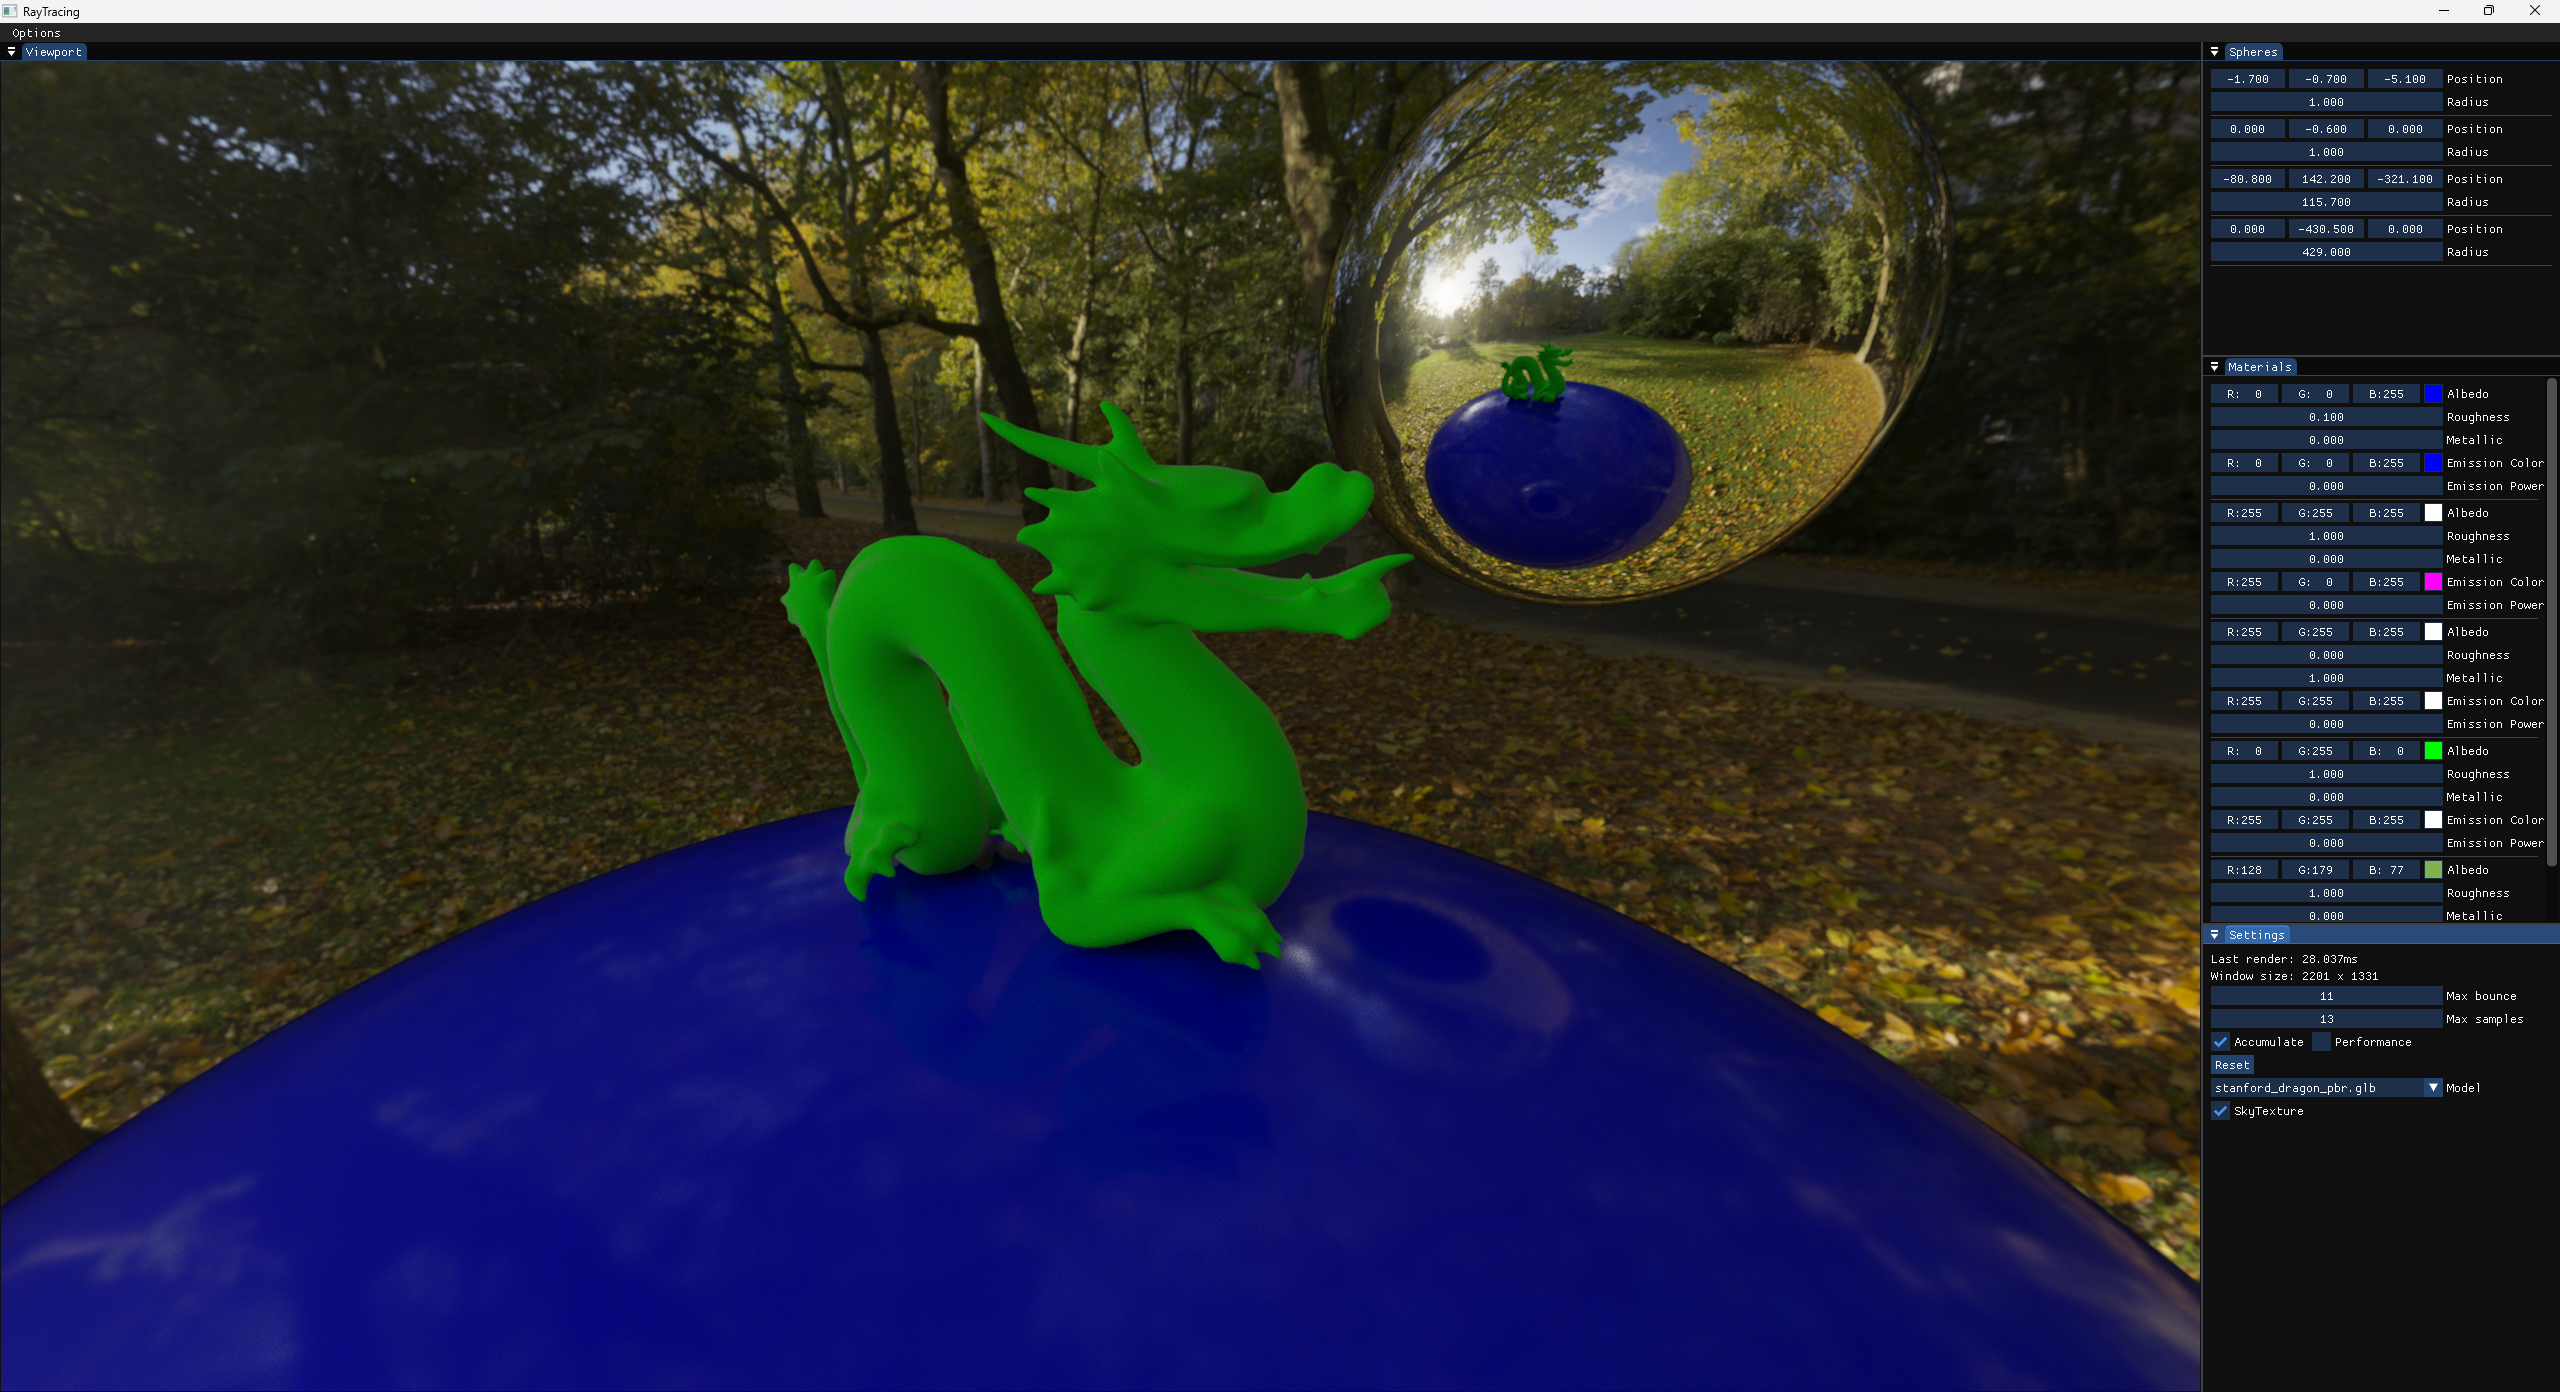
\includegraphics[width=0.8\textwidth]{Interfejs} 
    \caption{Zdjęcie przedstawia interfejs silnika.}
    \label{fig:interfejs}
\end{figure}

\section{Opis potoku graficznego}
\section{Implementacja algorytmów}